\chapter{Differential Equations}
\section{First Order D.E.s}
\subsection{Elementary Solving Techniques}
\begin{stbox}{General Information}
  \begin{itemize}
    \item Separable Variables:
    \begin{align*}
      \frac{dy}{dx}&=f(y)g(x),
      \int \frac{1}{f(y)}\,dy=\int g(x)\,dx.
    \end{align*}
    \item Integrating Factor:
    \begin{align*}
      \frac{dy}{dx}+P(x)y&=Q(x),\quad\text{let I.F.}=e^{\int P(x)\,dx}\\
      e^{\int P(x)\,dx} \frac{dy}{dx}+ye^{\int P(x)\,dx}P(x)&=Q(x)e^{\int P(x)\,dx},\\
      ye^{\int P(x)\,dx}&=\int Q(x)e^{\int P(x)\,dx}\,dx.
    \end{align*}
  \end{itemize}
\end{stbox}
\begin{example}{Justification for D.E. models of real world scenarios}{}
  Consider the proportion \(u\) of susceptible individuals --- those who have not yet caught the disease --- and the proportion \(v\) of infected individuals and the proportion \(w\) of recovered individuals. The standard model used in measuring the rate of spread of the disease assumes that \(du/dt=-kuv\), where \(k\) is a positive constant; the unit of time used is the average length of time for which a person is infected.
  \begin{enumerate}[label=(\alph*)]
    \item Describe the relevance of each bracketed term in the equation \(du/dt=(-k)(uv)\) in terms of the spread of the disease.
    \item Justify the assertion that \(dw/dt\approx v\).
  \end{enumerate}
  \rule{20cm-137.0549pt}{0.05mm} 
  \begin{enumerate}[label=(\alph*)]
    \item The \(uv\) term measures the interaction between susceptibles and infected. This should be directly proportional to \(du/dt\): When interactions between susceptibles and infected are more common (\(uv>0\) is larger), more susceptibles should become infected (\(du/dt\) is more negative). The proportionality constant \(-k\) between \(uv\) and \(du/dt\) is negative to illustrate this relationship; the proportion of susceptibles cannot increase when population size is constant.   
    \item Since the unit of time used in the model is the average length of time for which a person is infected, if there are \(I\) infected individuals at time \(t\), then after one unit time, roughly \(I\) people would have recovered. i.e. \(dR/dt\approx I\) so \(dw/dt\approx v\), where \(R\) is the number of people who have recovered.
  \end{enumerate}
\end{example}
\subsection{Numerical Methods}
\begin{stbox}{General Information}
  \begin{itemize}
    \item Euler's Method: 
    \[y_{i+1}=y_i+hf(x_i,y_i),\text{ where }x_n=x_0+nh.\]
    We can present our working directly, as shown in Example 17.1, if there are only one or two iterations. Otherwise, draw the following table.
    \begin{table}[H]
      \centering
      \begin{tabular}{|Sc|Sc|Sc|}
        \hline
        \(x\) & \(y\) & \(y+hf(x,y)\)\\
        \hline
        \(x_0\)& \(y_0\) & \(y_1\)\\
        \hline
        % \(x_0+h\)& \(y_1\) & \(y_2\)\\
        % \hline
        \(\vdots\) & \(\vdots\) & \(\vdots\)\\
        \hline
        \(x_n\) & \(y_n\) &\\
        \hline
      \end{tabular}
      \caption{Tabular presentation for Euler's Method.}
      \label{table:euler-presentation}
    \end{table}
  \end{itemize}
\end{stbox}
    \begin{example}{}{}
      Let (step size) \(h=0.25\) and \(f(x,y)=\frac{dy}{dx}\):
      \begin{align*}
        \text{By MF26,}\quad y_2&=\frac{2}{3}+hf\left(0,\frac{2}{3}\right)\\
        &=\frac{13}{18}\\[3mm]
        y_3&=\frac{13}{18}+hf\left(0.25,\frac{13}{18}\right)\\
        &=0.6701865657.\\[3mm]
        \text{Therefore, }y(0.5)&\approx 0.670.
      \end{align*}
    \end{example}
    \begin{stbox}{}
      \setcounter{enumi}{1}
    \begin{itemize}
    \item Improved Euler's Method: 
    \[u_{i+1}=y_i+hf(x_i,y_i)\quad\&\quad y_{i+1}=y_i+\frac{h}{2}[f(x_i,y_i)+f(x_{i+1},u_{i+1})].\]
    Usually only one or two iterations is necessary, so presenting our working directly is sufficient.
% \end{itemize}
% \begin{itemize}
    \item Error:
    \begin{enumerate}
      \item If \(\frac{dy}{dx}\) can be shown to be \emph{increasing} from the calculations of \(f(x,y)\), then the curve is \emph{concave upwards}, leading to a \emph{underestimate}.
      \item If \(\frac{dy}{dx}\) can be shown to be \emph{decreasing} from the calculations of \(f(x,y)\), then the curve is \emph{concave downwards}, leading to a \emph{overestimate}.
    \end{enumerate}
  \end{itemize}
\end{stbox} ~
\begin{example}{}{}
  From the computation, \emph{the values of} \(\frac{dy}{dx}\) \emph{increases}, i.e. \(\frac{d^2y}{dx^2}>0\), implying that the solution curve is \emph{concave upwards}. Therefore, we have an \emph{underestimation}. 
\end{example}
\begin{example}{}{}
  It is suggested that the estimation in part (ii)\footnote{Given the point (1,1), we estimated the value of y(2) using the Improved Euler's Method} can be further improved by reducing the step size. Sketch the solution curve and hence comment on this suggestion.\\[3mm]
  The solution curve has a \emph{stationary point at} \(x=1.47\), which is between 1 and 2 and also the gradient of the curve is close to zero for \(x\) value beyond this stationary point. Thus, when the step size is reduced, \emph{tangent} at point close to this stationary point becomes \emph{almost parallel} to the curve, making \emph{little improvement} to the estimation due to \emph{little difference in} \(y\). 
\end{example}
\begin{example}{}{}
  It is found that the approximation obtained in (i) for the \(y\)-coordinate where \(x=0.75\) is an underestimation and has a percentage error of 120.633\%. Explain why there is such a substantial error.\\[3mm]
  From gradient values calculated above, we suspect sharp charges in gradient values within the interval (from negative to positive). Yet \emph{Euler's Method\footnote{We are explaining what it does} simply uses a straight line segment} with gradient\footnote{Emphasising negative gradient (Show its value)} \(-4.6409\) to estimate the curve for the first iteration, which could have lead to a significant underestimation of the \(y\)-value.
\end{example}
\begin{note}{}{}
  Compare the relative merits of Euler's Method and the Improved Euler's Method.
  \begin{enumerate}[wide=0pt, leftmargin=*]
    \item[Euler's Method:] It is computationally simpler.
    \item[Improved Euler's Method:] It is More accurate as it takes the mean of the initial and next gradient. 
  \end{enumerate}
\end{note}
\begin{figure}[H]
  \centering
  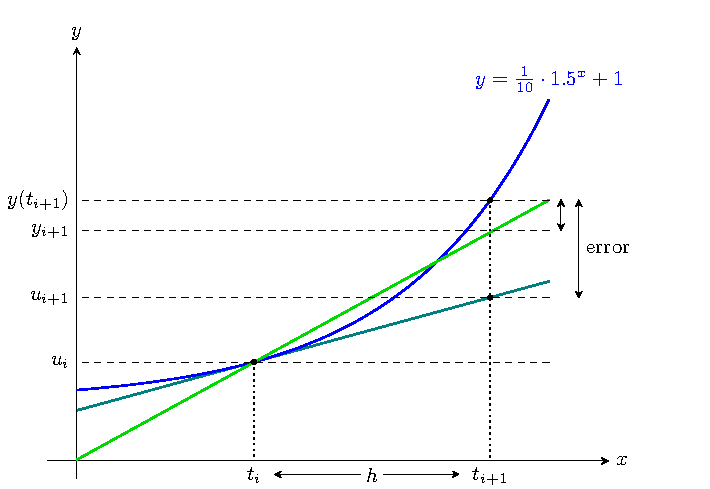
\includegraphics{../Diagrams/Euler's-Methods/euler's-method.pdf}
  \caption{\ref{source:euler's-methods} An illustration of \textcolor{green!50!blue}{Euler's Method} and the \textcolor{green!85!black}{Improved Euler's Method}.}
  \label{fig:euler's-methods}
\end{figure}
\begin{note}
  To find the percentage difference of the true value and the estimated value, we calculate
  \[\frac{\text{true value}-\text{estimated value}}{\text{true value}}\cdot 100\%.\]
\end{note}
\begin{note}
  Explain the large discrepancy between the approximations yielded by Euler's Method and the Improved Euler's Method.
  \begin{itemize}
    \item There is a large increase in the gradient of the curve from [the value of \(y'(a)\)] at \(x=a\) to [the value of \(y'(b)\)] at \(x=b\). 
    \item So, the average of the two gradients used in the Improved Euler's Method is significantly larger than [the value of \(y'(a)\)] used in Euler's Method.
    \item Hence, a large discrepancy between the results of the two methods is observed.
  \end{itemize}
\end{note}
\begin{note}
  State the condition when the Improved Euler's Method is not an improvement over Euler's Method
  \begin{center}
    When the gradient function is a constant throughout the allocated interval.
  \end{center} 
\end{note}
\begin{example}{Comparing three sets of approximations.}{}
  \begin{enumerate}[label=(\roman*)]
    \item Obtain the solution of the differential equation 
    \[\frac{dy}{dx}-y=x\]
    given that \(y=0\) when \(x=0\). Obtain, correct to 3 significant figures, the values of \(y\) when \(x=0.1\) and \(x=0.2\).
  \end{enumerate}
  Now consider the differential equation
  \[\frac{dy}{dx}-\sin(y)=x,\]
  where \(x=0\) when \(x=0\).
  \begin{enumerate}[label=(\roman*)]
    \setcounter{enumi}{1}
    \item Use Euler's Method with step length 0.1 to estimate the values of \(y\) when \(x=0.1\) and \(x=0.2\).
    \item Use the improved Euler Method with step length 0.1 to estimate the values of \(y\) when \(x=0.1\) and \(x=0.2\).
    \item Comment on your numerical answers from parts (i), (ii), and (iii). \hspace*{\fill} [2]
  \end{enumerate}
  \rule{20cm-137.0549pt}{0.05mm}
  \begin{enumerate}[label=(\roman*)]
    \item \(y(0.1)=0.00517\) and \(y(0.2)=0.0214\).
    \item \(y(0.1)\approx 0\) and \(y(0.2)\approx 0.01\).
    \item \(y(0.1)\approx 0.005\) and \(y(0.2)\approx 0.210\).
    \item 
    \begin{itemize}
      \item Since the values of \(y\) are small, \(\sin(y)\approx y\) by small angle approximation. \hspace*{\fill} [1]
      \item Hence, the values of \(y\) from (i) can be compared with estimates from (ii) and (iii). 
      \item Since the answers from (iii) are closer to those in (i) than the those in (ii), the answers in (iii) are more accurate estimates of the exact values of \(y\). \hspace*{\fill} [1]
    \end{itemize}
  \end{enumerate}
\end{example}
\begin{example}{}{}
  The function \(y=y(x)\) satisfies \(\frac{dy}{dx}=\frac{1}{10}(\sin(x)-xy)\). 
  \begin{enumerate}[label=(\roman*)]
    \item The value of \(y(h)\) is to be found, where \(h\) is a small positive number, and \(y(0)=0\).
    \begin{enumerate}
      \item Use two steps of Euler's method to determine an approximation to \(y(h)\) in terms of \(h\).
      \item Use one step of the improved Euler formula to find alternative solutions to \(y(h)\) in terms of \(h\).
    \end{enumerate}
    \item \textcolor{yellow}{\(\bigstar\)} Show that \(y=y(x)\) satisfies \(e^{0.05h^2}y(h)=\int_{0}^{h}0.1e^{0.05x^2}\sin(x)\,dx\).
    % \begin{align*}
    %   \frac{dy}{dx}&=\frac{1}{10}[\sin(x)-xy]\\
    %   \frac{dy}{dx}+\left( \frac{1}{10}x \right)&=\frac{1}{10}\sin(x)\\
    %   \text{Let I.F. be }e^{\int\frac{1}{10}x\,dx}&=e^{0.05x^2}:\\
    %   e^{0.05x^2}y&=\int\frac{1}{10}e^{0.05x^2}\sin(x)\,dx\\
    %   \left[e^{0.05x^2}y\right]_{0}^{h}&=\int_{0}^{h}\frac{1}{10}e^{0.05x^2}\sin(x)\,dx\\
    %   e^{0.05h^2}y(h)-e^0y(0)&=\int_{0}^{h}\frac{1}{10}e^{0.05x^2}\sin(x)\,dx\\
    %   \text{Since y(0)=0},\\
    %   e^{0.05h^2}y(h)&=\int_{0}^{h}\frac{1}{10}e^{0.05x^2}\sin(x)\,dx.
    % \end{align*}
    \begin{proof}
      We see that
      \begin{align*}
        \frac{dy}{dx}&=\frac{1}{10}[\sin(x)-xy]\\
        \frac{dy}{dx}+\left( \frac{1}{10}x \right)&=\frac{1}{10}\sin(x)\\
        \intertext{Let I.F. be \(e^{\int\frac{1}{10}x\,dx}=e^{0.05x^2}\):}
        e^{0.05x^2}y&=\int\frac{1}{10}e^{0.05x^2}\sin(x)\,dx\\
        \left[e^{0.05x^2}y\right]_{0}^{h}&=\int_{0}^{h}\frac{1}{10}e^{0.05x^2}\sin(x)\,dx\\
        e^{0.05h^2}y(h)-e^0y(0)&=\int_{0}^{h}\frac{1}{10}e^{0.05x^2}\sin(x)\,dx\\
        \shortintertext{Since \(y(0)=0\),}
        e^{0.05h^2}y(h)&=\int_{0}^{h}\frac{1}{10}e^{0.05x^2}\sin(x)\,dx.
      \end{align*}
    \end{proof}
    \item Use the fact that \(h\) is small to estimate \(\int_{0}^{h}0.1e^{0.05x^2}\sin(x)\,dx\). Hence find another approximation to \(y(h)\) in terms of \(h\).
    \item \textcolor{yellow}{\(\bigstar\)} Discuss the relative merits of the three methods employed to obtain these approximations.
  \end{enumerate}
  \begin{itemize}
    \item Two step of Euler's method might be lead to a more accurate approximation than one step of the improved Euler method, because of the larger number of steps.
    \item The improved Euler method might lead to a more accurate approximation, as it takes the mean of the gradients \(y'(0)\) and \(y'(h)\), rather than the simplistic tangent line approximation used by Euler's method.
    \item The method in (iii) might be more accurate than Euler's method and the improved Euler method, because it uses quadratic polynomials/an exponential curve\footnote{It depends on how you calculated the approximation to \(y(h)\) in (iii).} instead of straight line segments.
  \end{itemize}
\end{example}
\section{Second Order D.E.}
\begin{center}
  \begin{tabular}{|Sc|Sc|}
    \hline
    \multicolumn{2}{|Sc|}{\textbf{Homogenous}}\\
    \hline
    Roots & Solution \(y_c\)\\
    \hline
    \(m_1 \neq m_2\) & \(y=Ae^{m_1x}+Be^{m_2x}\)\\
    \hline
    \(m\coloneq m_1=m_2\) & \(y=(Ax+B)e^{mx}\)\\
    \hline
    \(m=\highlight[red!30]{p} \pm qi\) & \(y=e^{\highlight[red!30]{p}x}(A \cos(qx)+B \sin(qx))\)\\
    \hline
    \multicolumn{2}{|Sc|}{\textbf{Non-Homogenous, }\(c_2 \dfrac{d^2y}{dx^2}+c_1 \dfrac{dy}{dx}+c_0y=f(x)\)}\\
    \hline
    \multicolumn{2}{|Sc|}{\(y=y_c+y_p\) (C.F. + P.I.)}\\
    \hline
    \(f(x)\) & Trial Function for P.I.\\
    \hline
    Degree \(n\) polynomial & \(y_p=\sum\limits_{i=0}^{n}a_ix^i\)\\
    \hline
    \(\alpha e^{kx}\) & \(y_p=ae^{kx}\)\\
    \hline
    \(\alpha \cos(kx) +\beta \sin(kx)\) & \(y_p=a\cos(kx)+b\sin(kx)\)\\
    \hline
  \end{tabular}
  \begin{note}
    If \(y_c\) and \(f(x)\) share some common term, then \(y_p\) should be multiplied by \(x\) (some least \(i \in \mathbb{N}\) times till \(x^iy_p\) has no common term with \(y_c\)).  
  \end{note}
  \begin{example}{}{}
    \begin{enumerate}
      \item If \(y_c=Ae^{-3x}\) and \(f(x)=10e^x\), then \(y_p=ke^x\)
      \item If \(y_c=Ae^x+Be^{-3x}\) and \(f(x)=10e^x\), then \(y_p=kxe^x\).
      \item If \(y_c=Ae^x+Bxe^{x}+Ce^{-3x}\) and \(f(x)=10e^x\), then \(y_p=kx^2e^x\).
    \end{enumerate}
  \end{example}
\end{center}
\begin{note}\hypertarget{R-formulas}{}
  \(R\)-formulas. Let \(a,b\in \mathbb{R}\). Then, for 
  \[R\coloneq\sqrt{a^2+b^2} \qquad\text{and}\qquad \tan(\alpha)\coloneq\frac{b}{a},\]
  we have that
  \[a\sin(\theta)+b\cos(\theta)=R\sin(\theta+\alpha) \qquad\text{and}\qquad b\sin(\theta)+a\cos(\theta)=R\cos(\theta-\alpha).\]
\end{note}
\section{Applications}
\subsection{Exponential Growth}
\begin{stbox}{General Information}
  Let \(k\) be the \emph{per-capita growth rate}\footnote{i.e. after accounting for births and deaths.} and \(P(t)\) be the population at time \(t\). Then we have the model:
  \[\frac{dP}{dt}=kP,\]
  with the solution
  \[P(t)=P_0e^{kt}.\]
\end{stbox}
\subsection{Logistics Growth}
\begin{stbox}{General Information}
  Let \(k\) be the \emph{per-capita growth rate}\footnote{i.e. after accounting for births and deaths.}, \(P(t)\) be the population at time \(t\), and \(N\) be the \emph{carrying capacity} of the system. Then we have the model:
  \[\frac{dP}{dt}=kP\left(1-\frac{P}{N}\right).\]
  \begin{enumerate}
    \item Without solving the logistics equation, we can sketch the solution curve by noting the sign of \(dP/dt\):
    \begin{enumerate}
      \item Equilibrium population values occur at \(P=0\) and \(P=N\).
      \item If, for instance \(k>0\),
      \begin{enumerate}[wide=0pt, leftmargin=*]
        \item[\(0<p<N\):] \(1-\frac{P}{N}>0\) so \(dP/dt>0\),
        \item[\(P>N\):] \(1-\frac{P}{N}<0\) so \(dP/dt<0\).  
      \end{enumerate}
    \end{enumerate}
    ``As \(t\) increases,  the population of \rule{1cm}{0.1mm}  increases to the stable population of \rule{1cm}{0.1mm}.''
  \end{enumerate}
\end{stbox}
\begin{example}{Neat trick of letting \(A=\pm \text{constant}\)}{}
  \begin{align*}
    \frac{dP}{dt}&=3P\left(1-\frac{P}{200}\right),\\
    \int \frac{1}{3P}+\frac{1}{600-3P}\,dP &= \int 1 \,dt,\\
    \ln \abs{\frac{3P}{600-3P}}&=3t+3c,\\
    \frac{3P}{600-3P}&=Ae^{3t}\text{, where }\highlight[red!30]{A=\pm e^{3c}},\\
    P&=\frac{200A}{A+e^{-3t}}
  \end{align*}
\end{example}
\begin{figure}[H]
  \centering
  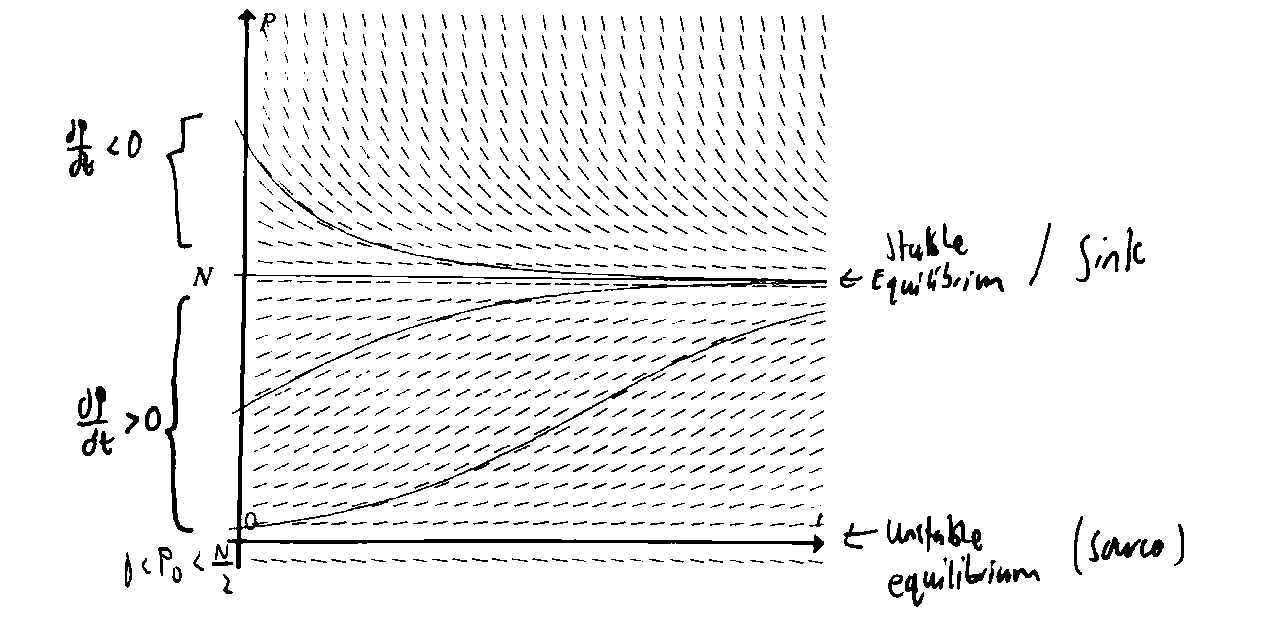
\includegraphics[width=0.35\textwidth]{Logistics Curve}
  \caption{\ref{Me} Logistics Curve}
  \label{fig:logistics-curve}
\end{figure}
\subsection{Harvesting}
\begin{stbox}{General Information}
  Let \(k\) be the \emph{per-capita growth rate}, \(P(t)\) be the population at time \(t\), \(N\) be the \emph{carrying capacity} of the system, and \(H\) the constant \emph{harvesting rate}. Then we have the model:
  \[\frac{dP}{dt}=kP\left(1-\frac{P}{N}\right)-H.\]
\begin{enumerate}
  \item Bifurcation Point
  \begin{enumerate}
    \item When \(0 \leq H<\frac{kN}{4}\), there are two equilibrium points, \(P=\frac{N}{2}\pm \sqrt{\frac{N^2}{4}-\frac{HN}{k}}\).
    \item When \(H=\frac{kN}{4}\), there is one equilibrium point at \(P=\frac{N}{2}\) (the bifurcation point).
    \item When \(H>\frac{kN}{4}\), there is no equilibrium point
  \end{enumerate}
  \item For Non-Extinction: 
  \begin{align*}
    \quad\frac{N^2}{4}-\frac{HN}{k} \geq 0 \qquad\text{and}\qquad P_0 \geq \frac{N}{2}-\sqrt{\frac{N^2}{4}-\frac{HN}{k}}.
  \end{align*}
\end{enumerate}
\end{stbox}

\subsection{Physics}
\begin{stbox}{General Information}
  \textbf{MUST} rmb the forms.
  \begin{enumerate}
    \item Spring System (where \(k>0\) is the spring constant) 
    \[\ddot{x}+\frac{k}{m}x=0.\]
    Solution: use \(\highlight[red!30]{\text{R-formula}}\) to convert to \(A \cos(\omega t + \phi)\) where angular frequency \(\omega=\sqrt{k/m}\). Period \(T=2\pi/\omega=2\pi \sqrt{m/k}\).
    \item Simple Pendulum (where \(\ell\) is its length)
    \[\ddot{x}+\frac{g}{\ell}x=0.\]
    Angular frequency \(\omega=\sqrt{g/\ell}\) and period \(T=2\pi \sqrt{\ell/g}\).
    \item Spring-Mass-Dashpot System (where \(c>0\) is the damping constant)
    \[\ddot{x}+\frac{c}{m}\dot{x}+\frac{k}{m}x=0.\]
    Solution
    \begin{enumerate}
      \item Real and Distinct Roots: \emph{Overdamped}
      \item Identical Real Roots: \emph{Critically Damped}
      \item Complex Conjugate Roots: \emph{Underdamped}\\
      \emph{``It will oscillate about the equilibrium position with decreasing amplitude.''}
    \end{enumerate}
  \end{enumerate}
\end{stbox}
\begin{figure}[H]
  \centering
  \includestandalone[width=\textwidth]{../Diagrams/Oscils}
  \caption{\ref{source:oscillatory-behavior} Oscillatory behaviors.}
  \label{fig:oscillatory-behavior}
\end{figure}